\documentclass{article}
\usepackage{graphicx} % Required for inserting images
\usepackage{amsmath}  % align environment for the DF-QuAD equations
\usepackage[hidelinks]{hyperref}
\usepackage[backend=biber, style=numeric]{biblatex}
\usepackage{booktabs}
\usepackage{tikz}
\usetikzlibrary{positioning,arrows.meta,fit,backgrounds}
\usepackage{listings}
\usepackage{seqsplit}                       % in preamble
\newcommand{\flag}[1]{\texttt{\seqsplit{#1}}}
% then:  \flag{--new-nodes}
\lstset{
  basicstyle=\ttfamily\small, % Uses typewriter font and makes it slightly smaller
  breaklines=true,             % Automatically wraps long lines
  breakatwhitespace=true,      % Prefers to break lines at spaces
  columns=fullflexible,        % Keeps spacing looking natural
  keepspaces=true,
  escapechar=|
}
\title{EpistemicCaseStudyCompetition}
\author{
  Amir Basareh$^{*}$ \quad Nathan Reed$^{*}$ \quad Arpita Saha$^{*}$\\[2pt]
  \small \texttt{abasareh@purdue.edu} \quad \texttt{nnreed@purdue.edu} \quad \texttt{saha119@purdue.edu}\\[4pt]
  \small $^{*}$All authors contributed equally.
}
\date{July 2026}
\bibliography{references}

\begin{document}

\maketitle

% \section{Introduction}

% We are introducing a system that takes documents and produces a Knowledge Graph taking cues from first-order logic. This graph, grounded in concepts from first-order logic, such as premise-conclusion format, will help us answer queries in epistemic case studies. The knowldege graph will represent facts and information from multiple documents, which will lead to the formation of more complete answers, backed by facts and data from paragraphs across different sources. Currently, LLMs are still unable to perform information retrieval across multiple documents with reliable accuracy. Due to catastrophic forgetting, performance of information linking across sentences or paragraphs in different documents suffers. Hence, we will make use of a non-parametric memory that updates graph nodes and edges as new data is fed into it in a continual learning manner and thus enhances the performance of an LLM's query retrieval as it goes along.    

\section{Introduction}
Large Language Models (LLMs) have demonstrated impressive capabilities in document understanding, summarization, and question answering. However, they still struggle when knowledge is distributed across multiple documents and must be synthesized into a coherent, evidence-backed response. In particular, LLMs often fail to consistently retrieve and connect information scattered across different sources, leading to incomplete reasoning, hallucinations, or contradictory conclusions. These limitations become even more pronounced in domains such as epistemic case studies, where conclusions must be justified by tracing chains of evidence spanning multiple documents, reports, or research papers.

The questions that matter in an epistemic case study--- \emph{what is the
evidence for this hypothesis}, \emph{where do the sources disagree}, and
\emph{which single assumption is the conclusion most sensitive to} --- are
questions about the structure of an argument, not about topical similarity. A
retriever that ranks passages by how much they mention a topic cannot tell a
supporting fact from a rebuttal, nor trace a conclusion back through the premises
it rests on.

Our central design commitment is therefore to make argumentative structure a
first-class, queryable object: a typed graph whose nodes are hypotheses, evidence,
assumptions, and claims, and whose relations are explicit \emph{support} and
\emph{attack} links, each grounded in an exact span of a source document. Nothing in the graph or query path is hard-coded to any one document; all
document-specific knowledge lives in configuration.

\section{System Design}

Our goal is a system that finds scientific information efficiently and reports
it accurately, with every answer traceable to the source it came from. Standard
retrieval systems, including HippoRAG~2~\cite{gutierrez2025rag} and GraphRAG~\cite{edge2024graphrag}, match a query to passages
or entity neighborhoods by topical similarity, extracting relations of the form
``\emph{X}---related to---\emph{Y}.'' That is enough to locate where a topic is
discussed, but not to answer the questions that matter in a scientific or
evidentiary case: what evidence supports a given claim, where two sources
disagree, or which assumption a conclusion most depends on. These are questions
about how claims relate to one another---often across documents---and a ranked
list of passages does not encode those relations, leaving the language model to
reconstruct them at answer time.

We therefore represent a document not as a set of passages but as an argument
graph built from three kinds of objects. \emph{Nodes} are atomic statements
extracted from the text, typed into three layers: \emph{data} (measurements,
statistics, experimental results), \emph{argument} (claims, interpretations,
rebuttals), and \emph{question} (hypotheses, conclusions). Each node carries a
byte-exact quote locating it in its source and receives a strength score in
$[0,1]$ computed over the whole graph. \emph{Cards} are the relations: a card
takes one or more premise nodes and one target node, labeled \emph{support} or
\emph{attack}---the structure of a bipolar argumentation framework.
Allowing several premises lets a card express a \emph{joint} argument:
``the trial was industry-funded'' attacks nothing on its own, and neither does
``industry-funded trials tend to overstate benefits,'' but together they attack
the trial's reliability. Much of the consequential argumentation in science,
law, and policy has exactly this shape, and a plain node-to-node edge cannot
represent it. \emph{Edges}, finally, carry no meaning of their own: they only
wire premises into cards, cards to their targets, and nodes to the documents
they came from.

Storing the argument structure explicitly has three practical payoffs. First,
\emph{accuracy}: each answer is assembled from specific nodes carrying exact
quotes, so it can be checked against the source rather than taken on trust.
Second, \emph{efficiency}: the expensive step---asking an LLM whether one node
supports or attacks another---is held to a fixed budget by a three-stage funnel
that blocks structurally implausible pairs by type, discards unrelated pairs
with an inexpensive filter, and sends only the top-ranked candidates to the
LLM, so labeling cost is capped regardless of corpus size; and because the
surviving relations are computed once, at ingestion, queries read stored
structure instead of re-analyzing text. Third, the graph is a
\emph{non-parametric memory}. Knowledge encoded in model parameters is
expensive to update and prone to catastrophic forgetting; here, adding a
document pairs its new nodes against the existing graph rather than rebuilding
it: duplicate claims are merged at extraction, new claims are added, and
contradictory evidence is recorded as attack cards rather than overwriting
what came before. Because every node keeps a source edge to its document, the
same machinery extends across documents: an evidence chain can aggregate
complementary findings from several sources, or surface exactly where they
conflict.

Once the cards are in place, no further LLM calls are needed on the graph side.
DF-QuAD~\cite{rago2016dfquad}, a gradual semantics for bipolar argument graphs, computes every
node's strength in a single pass in dependency order: supporters raise a
node's score and attackers lower it, each in proportion to its own strength.
The three query primitives read this structure directly. \emph{Evidence-for}
follows support cards inward from a claim and returns its premises, ranked by
strength. \emph{Contested} finds nodes carrying both support and attack cards
and reports which side is currently stronger. \emph{Weakest-link} removes each
card in turn, re-scores the graph, and reports the card whose removal moves
the conclusion most---the load-bearing link. The retrieved nodes' source
quotes, together with this structural answer, are then handed to an LLM, which
writes the prose response guided by the graph. The division of labor is
deliberate: the graph does the structural reasoning, the LLM does the reading
and explaining, and each layer can be audited independently. A response is
therefore not free text but a chain of support and attack steps, each grounded
in a quoted span of the original document---an advantage in epistemic case
studies, where \emph{why} a conclusion holds is often as important as the
conclusion itself.

Figure~\ref{fig:pipeline} shows the whole pipeline and how this report is
organized around it. It runs in three stages. \textbf{Claim extraction} turns each source PDF into typed, deduplicated claim nodes,
each carrying the exact quote and location it came from. \textbf{Knowledge
graph construction} (the next subsection) embeds those nodes, selects
candidate pairs through the funnel, labels each surviving pair as a support or
attack card, and scores every node with DF-QuAD. The \textbf{Query Engine}
(the subsection after that) then traverses the scored graph to answer a
question, returning a ranked chain of evidence with its sources rather than a
list of passages. The subsections below follow this order.

\begin{figure}[t]
\centering
\resizebox{\columnwidth}{!}{%
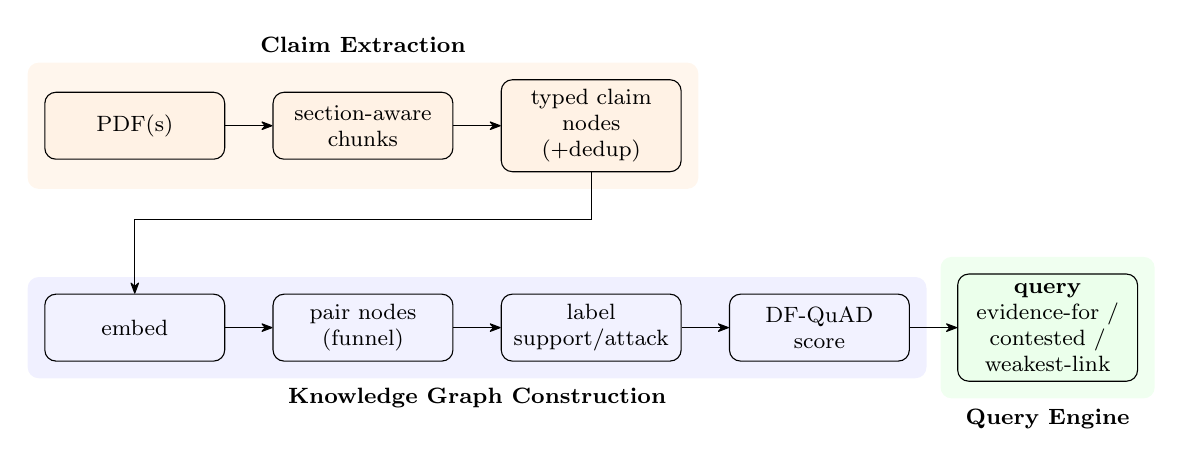
\begin{tikzpicture}[
  font=\footnotesize,
  >={Stealth[round]},
  stg/.style={draw, rounded corners, align=center, minimum height=0.85cm,
              text width=2.05cm, fill=blue!5},
  node distance=6mm and 6mm,
]
\node[stg, fill=orange!10] (pdf)     {PDF(s)};
\node[stg, fill=orange!10, right=of pdf]   (chunk)   {section-aware\\chunks};
\node[stg, fill=orange!10, right=of chunk] (extract) {typed claim\\nodes ($+$dedup)};
\node[stg, below=1.7cm of pdf]         (embed) {embed};
\node[stg, right=of embed]             (pair)  {pair nodes\\(funnel)};
\node[stg, right=of pair]              (label) {label\\support/attack};
\node[stg, right=of label]             (score) {DF-QuAD\\score};
\node[stg, fill=green!8, right=of score] (query)
     {\textbf{query}\\evidence-for /\\contested /\\weakest-link};
\draw[->] (pdf) -- (chunk);
\draw[->] (chunk) -- (extract);
\draw[->] (extract.south) -- ++(0,-0.6) -| (embed.north);
\draw[->] (embed) -- (pair);
\draw[->] (pair) -- (label);
\draw[->] (label) -- (score);
\draw[->] (score) -- (query);
\begin{scope}[on background layer]
  \node[rounded corners, fill=orange!7, fit=(pdf)(chunk)(extract),
        inner sep=6pt, label=above:{\textbf{Claim Extraction}}] {};
  \node[rounded corners, fill=blue!6, fit=(embed)(pair)(label)(score),
        inner sep=6pt, label=below:{\textbf{Knowledge Graph Construction}}] {};
  \node[rounded corners, fill=green!6, fit=(query),
        inner sep=6pt, label=below:{\textbf{Query Engine}}] {};
\end{scope}
\end{tikzpicture}%
}
\caption{The pipeline, and how the report maps onto it. \emph{Claim Extraction}
turns each PDF into typed claim nodes with exact-quote provenance;
\emph{Knowledge Graph Construction} embeds the nodes, connects and labels pairs
as support or attack cards, and scores every node with DF-QuAD; the \emph{Query
Engine} traverses the scored graph and returns a ranked, source-carrying
evidence chain. The multi-document extension stamps each node with its source
document, so the same flow answers cross-document questions.}
\label{fig:pipeline}
\end{figure}
% \section{System Design}


% To address this challenge, we introduce a knowledge graph construction framework inspired by principles of first-order logic. Existing retrieval systems such as HippoRAG and GraphRAG primarily model semantic relationships between concepts to identify relevant passages for retrieval. Although effective in locating information, they are less suited for answering questions that require reasoning about evidence distributed across multiple documents, such as identifying the evidence supporting a claim, locating contradictory findings across sources, or determining which assumption has the greatest impact on a conclusion. Rather than representing knowledge as isolated entities and relations, our system organizes information into logical structures resembling premise–conclusion reasoning. 
% % Each extracted statement is represented as a logical unit, where premises correspond to supporting evidence and conclusions represent claims or inferred knowledge. 
% This representation allows the graph to capture not only factual information but also the logical dependencies between pieces of evidence, creating a structured and explainable repository of knowledge.

% The proposed framework begins by processing a collection of documents and extracting semantically meaningful units such as facts, claims, hypotheses, assumptions, evidence, analyses, and conclusions. These units are transformed into canonical graph nodes, while logical relationships such as *supports*, *contradicts*, *explains*, *depends on*, or *implies* form the graph edges. Inspired by first-order logic, these relationships encode the reasoning process itself rather than merely recording co-occurrences between entities. Consequently, the resulting graph captures the underlying structure of arguments present across documents instead of simply storing disconnected facts.

% As additional documents are introduced, the graph evolves continuously. Newly extracted knowledge is compared against existing graph nodes through canonicalization and semantic matching. Equivalent concepts are merged, new facts are incorporated, contradictory evidence is explicitly represented, and relationships are updated without reconstructing the graph from scratch. This continual graph refinement enables the system to accumulate knowledge over time while preserving previously acquired information, effectively functioning as a growing repository of structured reasoning.

% A central motivation behind this work is overcoming the limitations of purely parametric memory in modern LLMs. Although LLMs encode enormous amounts of information within their model parameters, updating this knowledge typically requires expensive retraining or fine-tuning and often suffers from catastrophic forgetting, where newly learned information degrades previously acquired knowledge. Furthermore, parametric memory provides limited transparency, making it difficult to trace the origin of generated responses or verify whether conclusions are supported by evidence.

% Our approach instead leverages a **non-parametric memory** in the form of an evolving knowledge graph. Since knowledge is stored explicitly as graph nodes and logical relationships rather than implicitly within model parameters, new information can be incorporated incrementally without modifying the underlying language model. The graph therefore serves as an external memory that continually grows as new documents become available. Unlike neural memory, this external memory preserves historical information, enables explicit reasoning over accumulated evidence, and naturally supports continual learning.

% The explicit graph representation also enables reliable multi-document information retrieval. Traditional retrieval systems often return isolated document chunks that require the LLM to perform the integration internally. In contrast, our graph explicitly links related concepts originating from different documents, allowing the retrieval process to traverse logical chains connecting supporting evidence, intermediate conclusions, and final claims. As a result, the system can aggregate complementary information from multiple sources, reconcile overlapping evidence, identify conflicting viewpoints, and produce more comprehensive answers than retrieval methods operating on individual documents alone.

% The first-order logic-inspired organization of the graph further improves interpretability and explainability. Since each retrieved answer can be traced through a sequence of premise-to-conclusion relationships, users are able to inspect the reasoning path that produced a particular response. This provides an important advantage for epistemic case studies, where understanding *why* a conclusion was reached is often as important as the conclusion itself. Rather than producing opaque responses, the system offers evidence-backed reasoning grounded in the original documents.

\subsection{Claim Extraction}

We adapt our claim extraction system from the CAMS architecture proposed by Shuo Guan~\cite{guan_cams}, with additional support for node typing and a modified deduplication strategy. Our system begins by asking Meta-Llama 3.3 70b ~\cite{grattafiori2024llama3} Instruct-Turbo to extract, from each section of each document, a set of faithful, comprehensive, decontextualized, and atomic claim-nodes of some particular type. By faithful, we mean that the claim-nodes accurately represent the claims in the source document; by comprehensive, we mean that all relevant claims are extracted; by decontextualized, we mean that all pronouns, generic nouns, or abbreviations should be replaced by the corresponding full proper noun; and by atomic, we mean that each extracted claim-node should not be further separable into other claim-nodes. Faithfulness and comprehensiveness aim to ensure that future pipeline stages have a complete and accurate set of claims to begin with; decontextualization and atomicity ensure that future pipeline stages have the ability to operate on claim-nodes without significant further textual interpretation. The model is also asked to provide a source quote to support its extracted claim, and any claims with quotes that are not found in the text are removed from the pool, in order to ensure that claims are attributed to specific locations in the source document.

Since multiple types of nodes are extracted, the initial stage often creates duplicate nodes. These are subsequently filtered by checking for span overlap and text similarity, and merged if they are sufficiently similar (unless they fail the numeric conflict check, described shortly). Then, to filter duplicates across documents, all nodes not already merged are embedded using e5-instruct~\cite{wang2024multie5} prompted for equivalence, and the resulting cosine similarity matrix is used to generate candidate pairs for potential duplicate claims. Then, nli-deberta-v3-base~\cite{he2023debertav3} is used to ensure that both claims entail each other and do not contradict each other. This prevents claims with similar embeddings but contradictory meanings from being merged. Finally, even if the NLI model accepts a pair, a numeric conflict detector is run over the claims to ensure that claims using different numbers are not mistakenly merged. Once all potential duplications are checked, the longest claim-node text is chosen as the most representative row for further stages. Merges only occur if all nodes in a given cluster are linked, and otherwise fall back on the largest fully connected subset.

\subsection{Knowledge Graph Construction}

We build the graph in three steps: turn extracted claims into typed nodes,
connect related nodes with support or attack relations we call \emph{cards}, and
use those cards to compute a strength score for every node. This is one part of a
larger system --- extraction, querying, and evaluation are covered elsewhere in
this report --- and what follows describes a working prototype, not a finished
product.

\paragraph{Typed nodes.}
Every claim pulled from a document becomes a node. Each node records what kind of
statement it is, the exact quote and location it came from in the source text,
which document it came from, and how much we trust it (from a byte-exact quote
down to something the model inferred, without a supporting quote).

We sort nodes into ten types: hypothesis, evidence, estimate, assumption,
rebuttal, verdict, background, claim, subquestion, and correlation group. We then group them into three broader layers that the rest of the pipeline reasons about:

\begin{itemize}
    \item \textbf{Data}: raw observations, numbers, and context (evidence,
        estimates, background, correlation groups).
    \item \textbf{Argument}: interpretations and inferences built on that data
        (claims, rebuttals, assumptions).
    \item \textbf{Question}: what is actually being debated (hypotheses,
        verdicts, subquestions).
\end{itemize}

On our single-document test case, this produced \textbf{1{,}370 typed nodes}:
387 evidence, 365 claims, 314 background, 105 estimates, 75 assumptions, 53
hypotheses, 51 rebuttals, and 20 verdicts.

\paragraph{Cards: how nodes connect.}
Nodes are joined by \emph{cards}: labeled support or attack relations, each of
which may take several premises at once~\cite{cayrol2005baf,rago2016dfquad}. A
plain edge connects one node to one other; a card can combine multiple premises
into a single relation (Figure~\ref{fig:cards}), which is what joint arguments
require. We label cards by asking an LLM~\cite{gorur2024argmining}. On the
fixture this produced \textbf{1{,}253 cards}: 907 support, 346 attack. Our
labeler is pairwise, so every card built so far carries a single premise; the
multi-premise form is supported by the schema and by the scorer (a joint card
takes the strength of its weakest premise) but is not yet exercised.
 
\begin{figure}[t]
\centering
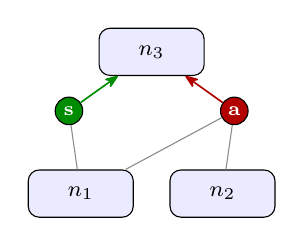
\begin{tikzpicture}[
  font=\footnotesize,
  >={Stealth[round]},
  nd/.style={draw, rounded corners, align=center, minimum height=0.6cm,
             text width=1.1cm, fill=blue!8},
  cd/.style={draw, circle, minimum size=3.5mm, inner sep=0pt,
             font=\scriptsize\bfseries},
]
\node[nd] (a) at (0,0) {$n_1$};
\node[nd] (b) at (1.8,0) {$n_2$};
\node[nd] (c) at (0.9,1.8) {$n_3$};
\node[cd, fill=green!55!black, text=white] (s) at (-0.15,1.05) {s};
\node[cd, fill=red!70!black, text=white]   (a2) at (1.95,1.05) {a};
\draw[-,black!45] (a) -- (s);
\draw[->,green!55!black,semithick] (s) -- (c);
\draw[-,black!45] (a) -- (a2);
\draw[-,black!45] (b) -- (a2);
\draw[->,red!70!black,semithick] (a2) -- (c);
\end{tikzpicture}
\caption{Two cards targeting $n_3$: a single-premise support (s) and a
joint attack (a) whose two premises combine into one relation. The joint form is
what the schema permits; the current build contains only single-premise cards.}
\label{fig:cards}
\end{figure}


\paragraph{Scoring the graph.}
Once the cards exist, we compute a strength score between 0 and 1 for every node
using a published method called DF-QuAD. The idea is intuitive: a node starts at
a neutral 0.5, its supporters push the score up, its attackers push it down, and
a joint card is only as strong as its single weakest premise. This step is pure
arithmetic --- no language model is involved --- and it is computed once across
the whole graph, working outward from the nodes that don't depend on anything
else. On the fixture, \textbf{93 nodes ended up ``contested''} --- carrying both
support and attack --- which is exactly the set of claims where the sources
genuinely disagree.

\paragraph{Deciding which pairs to check.}
The expensive step is deciding whether two nodes relate at all. Checking that
with a language model costs one call per pair, and the number of possible pairs
grows fast as the graph gets bigger. So we set a fixed budget on how many pairs
we are willing to check, and spend it on the pairs most likely to matter: we rule
out pairs that don't make structural sense (two pieces of raw data are unlikely
to directly attack each other; two hypotheses are compared, not connected), rank
what's left by how closely related the two nodes are, and send only the top
candidates to the model. This keeps the cost of building the graph roughly
constant whether the corpus has 500 nodes or 100{,}000 --- only how aggressively
we filter changes.

We also spend that budget unevenly, depending on direction:
\begin{itemize}
    \item \textbf{Top-down} (about half the budget): match each hypothesis with
        the data closest to it. This has the best hit rate.
    \item \textbf{Bottom-up} (most of the rest): connect data up to arguments,
        and arguments up to hypotheses, so a query can trace a full chain from
        raw fact to interpretation to hypothesis.
    \item \textbf{Contradiction} (a small slice): look within a layer for direct
        disagreements, using a small trained classifier rather than similarity
        search, since two similar-sounding claims can just as easily be
        contradicting each other as agreeing.
\end{itemize}

This split mattered in practice. Retyping misclassified interpretive conclusions
from data to argument (unblocking the bottom-up hop) and pairing them upward to
their hypotheses (closing the top-down hop) took our main evidence query from 7
one-hop summary leaves to 11 supporters over 22 raw data nodes at depth two ---
and revealed the leading hypothesis as contested rather than one-sidedly
supported.

\paragraph{Extending to multiple documents.}
Because every node already records which document it came from, this whole
process extends to more than one source without changing anything about the
underlying schema. When we add a second document, its nodes are paired against
the existing graph the same way, so if two independent sources agree on
something, that shows up as an explicit support relationship between them ---
not as a single node that silently absorbs both. We also use one model call per
document to identify which claims are genuinely top-level hypotheses, as opposed
to smaller sub-claims that happen to be phrased speculatively, so this step is
not tuned to any one document. Applied to two independent judges' rulings on the
same case (Eric's and Will's decisions), this produced a single graph of
\textbf{2{,}232 nodes} (2{,}077 from Eric's decision, 155 from Will's) connected
by \textbf{1{,}678 cards} (1{,}382 support, 296 attack), with four top-level
hypotheses identified automatically. Of those cards, \textbf{230 are
cross-document}, a premise in one judge's decision supporting or attacking a
claim in the other's, so agreement and disagreement between the judges become
explicit graph structure rather than something a reader must infer. \textbf{82
nodes are contested} (carrying both support and attack), and \textbf{31 of them
draw on both documents at once}: precisely the places where the two judges, or
the sources they cite, pull in opposite directions. Because every node is
document-attributed, asking for the evidence behind a shared hypothesis returns a
chain grouped by document, for the hypothesis that an animal host at the Huanan
Seafood Market caused the outbreak, 47 supporting premises, 45 from Eric and 2
from Will.


\subsection{Query Engine}

% \paragraph{Full-graph scans (no target node).}
% \begin{description}
%     \item[\texttt{contested}] Nodes with both supporters and attackers, ranked by how lopsided the disagreement is.
%     \item[\texttt{rank-hypotheses}] Every hypothesis-type node, sorted by DF-QuAD strength.
%     \item[\texttt{quantitative-backbone}] Every estimate-type node (the numeric core of the argument) and what it feeds into.
% \end{description}

% \paragraph{Unfiltered traversal.}
% \begin{description}
%     \item[\texttt{evidence-for}] Support-only chain from a target node, any type, returned as a nested tree; groups by source document when the chain spans more than one.
% \end{description}

% \paragraph{Type-filtered, polarity-split.}
% Each walks \emph{both} the support and attack chain of a target node,
% filtered to one node type, with polarity flipping across every attack edge
% (something supporting an attacker still counts against the target).
% \begin{description}
%     \item[\texttt{claims-for}, \texttt{background-for}, \texttt{evidence-only-for}, \texttt{assumptions-for}, \texttt{rebuttals-for}, \texttt{verdicts-for}] One per real node type.
%     \item[\texttt{analysis-for}, \texttt{limitations-for}] Same mechanism; always empty on real data since ``analysis''/``limitation'' are not current node types.
%     \item[\texttt{quantitative-evidence-for}] Filtered to numeric nodes, enriched with the extracted number and its attribution.
% \end{description}

% \paragraph{Polarity-only, unfiltered by type.}
% \begin{description}
%     \item[\texttt{supporting-for}, \texttt{negating-for}] All nodes of any type on one side of the argument.
% \end{description}

% \paragraph{Ablation-based.}
% \begin{description}
%     \item[\texttt{weakest-link}] Removes each card in the corpus one at a time and rescores the whole graph, ranking by impact on a target node's strength.
%     \item[\texttt{weakest-link-scoped}] Identical results, restricted to cards within the target's own dependency closure for efficiency.
% \end{description}


A knowledge graph built only from generic entity--relation triples (as in
HippoRAG-style retrieval) can locate topically relevant passages but cannot
answer questions that require argumentative structure: what supports a
claim, where the evidence conflicts, or which single piece of evidence a
conclusion actually depends on across the same or different documents. We address this by scoring every node with
DF-QuAD and exposing that structure through fourteen query operations,
organized into five families.


\subsection{Graph Traversal Techniques for different Query Types}
Our technique uses the following graph traversal algorithms for the different types of queries:
\paragraph{Dependency-ordered scoring.} Every node's DF-QuAD strength depends
recursively on the nodes feeding its incoming relations, so scores must be
computed in an order that respects this dependency. We condense the
relation graph into strongly connected components via Tarjan's algorithm,
which yields components already in evaluation order: no component is
visited before every component it depends on. Acyclic components are scored
in a single pass; genuine cycles (mutually reinforcing or conflicting nodes)
are initialized at the base strength and iterated to a fixed point. This is
the one traversal that produces structure rather than consuming it -- every
technique below operates on the supporter/attacker relations this pass
establishes.

\paragraph{Signed bidirectional traversal.} Answering ``what supports or
undermines this node'' requires following both supporting and attacking
relations backward from a target while tracking whether each path
ultimately argues for or against it. We perform a memoized depth-bounded
walk that carries a polarity value, inverted at every attacking relation and
preserved across every supporting one, so a node reached through an even
number of attacking hops is correctly classified as supporting and an odd
number as negating. Memoization is keyed on the (node, polarity) pair rather
than the node alone, since the same node can legitimately be reached at both
polarities via independent paths. Type filtering, where applied, is a
post-hoc predicate on visited nodes rather than a pruning rule -- the walk's
cost depends on the size of the reachable region, not on how rare the
target type is.

\paragraph{Unfiltered tree recovery.} The base evidence traversal follows
only supporting relations and preserves the path structure explicitly,
returning a nested tree rather than a flattened set, so a multi-step
support chain is recoverable as such rather than collapsed into an
unordered list. A second, structural pass over the completed tree detects
whether it spans more than one source document and, if so, discards the
nesting in favor of grouping by document -- a shape transformation applied
after traversal, not an alternative search strategy.

\paragraph{Bounded reachability for targeted ablation.} Determining which relation is most load-bearing for a conclusion naively requires rescoring the entire graph once per relation in the corpus, the large majority of which cannot possibly affect a given target. Since strength propagates in only one direction through the relation graph, we first compute the complete backward-reachable closure of relations from the target -- with no depth bound, since correctness here requires certainty that nothing relevant is excluded -- and restrict ablation to that closure. This is a traversal used to safely shrink the input to an otherwise unmodified algorithm, yielding identical results at a fraction of the cost.

% \paragraph{Global scans.}
% These require no target node; they summarize the graph as a whole.
% \begin{description}
%     \item[\textsc{Contested}] Surfaces every node with both supporting and
%         attacking evidence, ranked by how decisively one side currently
%         dominates -- a direct answer to \emph{where do the sources disagree}.
%     \item[\textsc{Rank-Hypotheses}] Orders all competing top-level hypotheses
%         by their DF-QuAD strength, giving a single, evidence-weighted answer
%         to the document's central question.
%     \item[\textsc{Quantitative-Backbone}] Isolates the numeric core of the
%         argument -- priors, rates, Bayes factors -- and the claims each one
%         feeds into, separating quantitative reasoning from qualitative
%         narrative.
% \end{description}

% \paragraph{Unfiltered evidence traversal.}
% \begin{description}
%     \item[\textsc{Evidence-For}] Recovers the full support chain behind a
%         node as a ranked, nested tree, automatically regrouping by source
%         document when the chain spans more than one -- the base traversal
%         every type-specific query below specializes.
% \end{description}

% \paragraph{Type-filtered, polarity-aware traversal.}
% Each of these follows \emph{both} the supporting and attacking chain of a
% target node, narrowed to one epistemic role, with polarity inverted at every
% attack edge -- a node that bolsters an attacker of the target is correctly
% classified as working against it, not for it.
% % \begin{description}[style=unboxed]
% %     \item[\textsc{Claims-For}, \textsc{Background-For}, \textsc{Evidence-For}
% %         (typed), \textsc{Assumptions-For}, \textsc{Rebuttals-For},
% %         \textsc{Verdicts-For}] Recover exactly the claims, background facts,
% %         evidence, assumptions, rebuttals, or verdicts bearing on a target,
% %         split into those that support it and those that undermine it.
% %     \item[\textsc{Quantitative-Evidence-For}] The numeric analogue: returns
% %         only the quantitative claims bearing on a target, each annotated
% %         with its extracted value and attribution, split by polarity.
% % \end{description}
% \begin{description}
%     \item[\textsc{Qualitative Relations}] 
%         (\textsc{Claims-For}, \textsc{Background-For}, \textsc{Evidence-For} (typed), \textsc{Assumptions-For}, \textsc{Rebuttals-For}, \textsc{Verdicts-For}): 
%         Recover exactly the claims, background facts, evidence, assumptions, rebuttals, or verdicts bearing on a target, split into those that support it and those that undermine it.
        
%     \item[\textsc{Quantitative-Evidence-For}] 
%         The numeric analogue: returns only the quantitative claims bearing on a target, each annotated with its extracted value and attribution, split by polarity.
% \end{description}

% \paragraph{Polarity-only retrieval.}
% \begin{description}
%     \item[\textsc{Supporting-For}, \textsc{Negating-For}] Every node bearing
%         on a target, of any epistemic type, restricted to one side of the
%         argument -- the coarsest and cheapest way to ask ``what's the case
%         for'' or ``what's the case against.''
% \end{description}

% \paragraph{Sensitivity analysis.}
% \begin{description}
%     \item[\textsc{Weakest-Link}] Identifies the single most load-bearing
%         piece of evidence for a conclusion by ablating each relation in turn
%         and measuring the resulting shift in strength -- not the weakest
%         evidence in isolation, but the one whose removal changes the
%         conclusion the most.
%     \item[\textsc{Weakest-Link-Scoped}] An equivalent, more efficient
%         formulation that restricts ablation to the target's own dependency
%         closure, since relations outside it provably cannot affect its
%         score.
% \end{description}

\paragraph{Global scans.}
These require no target node; they summarize the graph as a whole.
\begin{itemize}
    \item \textbf{\textsc{Contested}:} Surfaces every node with both supporting and
        attacking evidence, ranked by how decisively one side currently
        dominates -- a direct answer to \emph{where do the sources disagree}.
    \item \textbf{\textsc{Rank-Hypotheses}:} Orders all competing top-level hypotheses
        by their DF-QuAD strength, giving a single, evidence-weighted answer
        to the document's central question.
    \item \textbf{\textsc{Quantitative-Backbone}:} Isolates the numeric core of the
        argument -- priors, rates, Bayes factors -- and the claims each one
        feeds into, separating quantitative reasoning from qualitative
        narrative.
\end{itemize}

%\paragraph{Unfiltered evidence traversal.}
% \begin{itemize}
%     \item \textbf{\textsc{Evidence-For}:} Recovers the full support chain behind a
%         node as a ranked, nested tree, automatically regrouping by source
%         document when the chain spans more than one -- the base traversal
%         every type-specific query below specializes.
% \end{itemize}

\paragraph{Type-filtered, polarity-aware traversal.}
Each of these follows \emph{both} the supporting and attacking chain of a
target node, narrowed to one epistemic role, with polarity inverted at every
attack edge -- a node that bolsters an attacker of the target is correctly
classified as working against it, not for it.
\begin{itemize}
    \item \textbf{\textsc{Qualitative Relations}} 
        (\textsc{Claims-For}, \textsc{Background-For}, \textsc{Evidence-For} (typed), \textsc{Assumptions-For}, \textsc{Rebuttals-For}, \textsc{Verdicts-For}): 
        Recover exactly the claims, background facts, evidence, assumptions, rebuttals, or verdicts bearing on a target, split into those that support it and those that undermine it.
        
    \item \textbf{\textsc{Quantitative-Evidence-For}:} 
        The numeric analogue: returns only the quantitative claims bearing on a target, each annotated with its extracted value and attribution, split by polarity.
\end{itemize}

\paragraph{Polarity-only retrieval.}
\begin{itemize}
    \item \textbf{\textsc{Supporting-For}, \textsc{Negating-For}:} Every node bearing
        on a target, of any epistemic type, restricted to one side of the
        argument.
\end{itemize}

\paragraph{Sensitivity analysis.}
\begin{itemize}
    \item \textbf{\textsc{Weakest-Link}:} Identifies the single most load-bearing
        piece of evidence for a conclusion by ablating each relation in turn
        and measuring the resulting shift in strength -- not the weakest
        evidence in isolation, but the one whose removal changes the
        conclusion the most.
    \item \textbf{\textsc{Weakest-Link-Scoped}:} An equivalent, more efficient
        formulation that restricts ablation to the target's own dependency
        closure, since relations outside it provably cannot affect its
        score.
\end{itemize}

\section{Qualitative Evaluation}

We compared our extraction results with the HippoRAG architecture proposed by \cite{gutierrez2025rag}. 

HippoRAG \cite{gutierrez2025rag} uses an LLM to perform OpenIE, extracting unconstrained (subject, relation, object) triples from documents. The subject and object phrases become nodes in a flat knowledge graph, while named entity recognition (NER) extracts entities from the query to identify retrieval seed nodes. The graph’s edges are labeled directly with the free-form relations produced by OpenIE, such as born in or part of, but it contains no higher-level hierarchy distinguishing claims, hypotheses, evidence, or other argumentative roles. Personalized PageRank then traverses this graph to retrieve information through multi-hop connections.





\subsubsection*{Analysis of Results}
Our evaluation of complex scientific evidence retrieval in Appendix \ref{Appendix} shows that the proposed graph-based system substantially outperforms HippoRAG by explicitly modeling the epistemic structure of scientific arguments. Whereas HippoRAG often relies on surface-level semantic similarity and struggles to retrieve direct evidence from dense or contradictory texts, the proposed architecture traverses multi-hop reasoning chains to recover precise claims and their supporting context. It also distinguishes the roles of retrieved information—such as supporting, opposing, or background evidence—while isolating specific molecular and historical details, including the DEFUSE proposal and WIV1 backbone data. This structured representation produces outputs that are more precise, verifiable, and contextually grounded than those obtained through standard semantic retrieval.

\section{Limitations and Future Work}
The system answers the epistemic queries it was designed for, reasons
\emph{across} documents, and, in our comparison, comes out ahead of the
baseline systems; what remains is scope we did not reach before the deadline
rather than dead ends. Both extensions below are ones the design already
anticipates.
\paragraph{Further improving claim extraction.}
While the claim extraction pipeline has managed to achieve fairly strong faithfulness (assessed qualitatively), it remains only somewhat comprehensive (as measured by the percentage of text spans captured in source quotes), and a few claim-nodes do still fail decontextualization and atomicity (as measured by the presence of generic nouns and conjunctions in claim-nodes). Further work would likely develop a postprocessing pipeline to extract more claims from unmined spans, as well as to decontextualize and atomize claims that are not yet decontextualized or atomized.
\paragraph{Fast/slow ingestion split.}
Ingestion has a cheap per-document pass (extract, type, embed, store) and an
expensive relational one (support/attack labeling and re-scoring); we
currently run them together. Splitting them would make a new document
queryable within seconds, with sparse answers that sharpen as a background
pass fills in the cards, and would keep LLM labeling off the critical path of
every query.
\paragraph{Incremental, online updates.}
The pieces already exist: the funnel's \flag{--new-nodes} mode pairs only
a new document's nodes against the existing graph, and DF-QuAD need only
re-score the affected sub-graph. Our two-document run is the first step of
exactly this---the second decision was paired against the first, earlier cards
persisting---and hardening it into one-document-at-a-time operation would let
the knowledge base grow continuously instead of being built in one shot.

\paragraph{Embedding-based Query Design.}
The current query engine performs exact graph traversal over explicitly defined relations, requiring user queries to be mapped to existing graph nodes before retrieval. While this enables precise and explainable reasoning, it limits the system's ability to handle free-form natural language queries that do not directly correspond to canonical node labels. Future work could use node embeddings to resolve free-text questions to graph nodes directly and thus allow extensive and flexible Natural Language query resolution.


% \subsection{Analysis of results}:
% Our evaluation of complex scientific evidence retrieval demonstrates that the proposed graph-based system significantly outperforms

\appendix
\section{Case Studies}
\label{Appendix}
\subsection{Case Study: Complex Evidence Retrieval (Node 00168) from "Eric\_Decision.pdf"}

\paragraph{Our System Output}
\begin{lstlisting}
|\normalfont\textbf{Node 00168 supporting evidence}|: The claim that "Rootclaim's claim is that the SARS-CoV-2 outbreak was due to gain-of-function laboratory research" (Section 1.3) is supported by several arguments. For instance, Rootclaim evaluates 80% of pandemics that first appear in Wuhan to be lab leaks, as stated in Section 3.2 of the document "eric_decision.pdf", which quotes "Similarly, Rootclaim evaluates 80% of pandemics that first appear in Wuhan to be lab leaks". Additionally, the primary case for the lab-leak hypothesis would be any laboratory worker at a lab doing gain-of-function research on coronaviruses, as mentioned in Section 4.2, quoting "ForLL, the primary case would be any laboratory worker at a lab doing gain-of-function research on coronaviruses".

Further support comes from the observation that the Project DEFUSE proposal matches features of SARS-CoV-2 (Section 7.6), with the document quoting "The centerpiece of the lab leak explanation is the Project DEFUSE proposal, and the observation that a number of features from that proposal match features of sars-cov-2:". The Project DEFUSE research plan also looks eerily similar to SARS-CoV-2 in parts (Section 7.2), as stated in the quote "The Project DEFUSE research plan [14, 20] looks eerily similar, in parts, to sars-cov-2". Other supporting points include SARS-CoV-2 first appearing in Wuhan, the same city as one of the labs involved in DEFUSE (Section 7.6), and SARS-CoV-2 having an FCS that looks artificially inserted when compared to banal-52 (Section 7.6).

Background information, such as Project DEFUSE involving the collection of bat coronaviruses and performing computer and lab testing on them (Section 5.4), and researchers at the WIV examining a preliminary sequence for SARS-CoV-2 by December 27, 2019 (Section 6), also provides context for the claim. However, it's noted that the results of the phylogenetic tree of the earliest COVID cases are not without dispute (Section 1.2.1), quoting "though the results are not without dispute".

|\normalfont\textbf{Node 00168 opposing evidence}|: The claim that "Rootclaim's claim is that the SARS-CoV-2 outbreak was due to gain-of-function laboratory research" (section 1.3) is negated by several arguments. One such argument is that "Rootclaim created a quantitative model to illustrate how an initial patient unassociated with HSM could yield the observed outbreak" (section 4.5.1), as stated in the document "eric_decision.pdf": "Rootclaim created a quantitative model ([5] at 2:29:40) to illustrate how an initial patient unassociated with HSM could yield the observed outbreak;" This suggests that there are alternative explanations for the outbreak that do not involve gain-of-function laboratory research. Additionally, the laboratory work involved editing a backbone of WIV1, a specific sars-like coronavirus genome chosen for its lack of pandemic potential (section 5.4.3), which is quoted as "In both cases the work involved editing a backbone of WIV1, a specific sars-like coronavirus genome chosen for its lack of 'pandemic potential'". Furthermore, the only SARS-CoV-2-like virus found by the group is RaTG13, which is neither a live virus nor the progenitor of SARS-CoV-2 (section C.1), as stated: "The only SARS-CoV-2-like virus found by this group is RaTG13, which is neither a live (cultured) virus nor the progenitor of SARS-CoV-2". These arguments collectively negate the claim that the SARS-CoV-2 outbreak was due to gain-of-function laboratory research.
\end{lstlisting}


\paragraph{HippoRAG Output}
\begin{verbatim}

{
    "question": "Rootclaim's claim is that the SARS-CoV-2 outbreak was due to 
                 gain-of-function laboratory research. What evidence supports 
                 this claim?",
    "answer": "None explicitly stated.",
    "gold_answers": null,
    "docs": [
      "Rootclaim's claim is that the SARS-CoV-2 outbreak was due to 
       gain-of-function laboratory research.\n\nQuote: \"Rootclaim's claim 
       that the sars-cov-2 outbreak was due to gain-of-function laboratory 
       research,\"",
      "The event that covid resulted as a lab-leak from a lab conducting 
       gain-of-function research is denoted as LL\n\nQuote: \"andLL be the 
       event that covid resulted as a lab-leak from a lab conducting 
       gain-of-function research\"",
      "The primary case for the lab-leak hypothesis would be any laboratory 
       worker at a lab doing gain-of-function research on coronaviruses\n\n
       Quote: \"ForLL, the primary case would be any laboratory worker at a 
       lab doing gain-of-function research on coronaviruses\"",
      "Rootclaim attempted to observe empirically how covid behaves by 
       introducing a list of known covid outbreaks in China centered at or 
       involving markets.\n\nQuote: \"Rootclaim attempted to do just that by 
       introducing a list of known covid outbreaks in China centered at or 
       involving markets ([5] at 2:21:50).\"",
      "Section 4 includes an extended discussion of Rootclaim's reasoning for 
       expecting a COVID-19 outbreak in the Huanan Seafood Market under the 
       lab leak hypothesis.\n\nQuote: \"This includes an extended discussion 
       of Rootclaim's reasoning for expecting a covid outbreak there under 
       the lab leak hypothesis.\""
    ]
  },
  {
    "question": "Rootclaim's claim is that the SARS-CoV-2 outbreak was due to 
                 gain-of-function laboratory research. What evidence negates 
                 this claim?",
    "answer": "The evidence that negates Rootclaim's claim includes the equal 
               consistency of observational evidence with zoonotic spillover, 
               the model's failure to explain early outbreak events, the 
               frontloading of HSM cases to earlier in the outbreak, and the 
               patterns observed in market-centered outbreaks.",
    "docs": [
      "Rootclaim believes the observational evidence is equally consistent with 
       zoonotic spillover anywhere in Wuhan as in HSM.\n\nQuote: \"as they 
       believe the observational evidence is equally consistent with zoonotic 
       spillover anywhere in Wuhan as in HSM,\"",
      "When the 2019 cases are broken down by time, Rootclaim's model does even 
       worse at explaining events earlier in the outbreak.\n\nQuote: \"When 
       the 2019 cases are broken down by time, the model does even worse at 
       explaining events earlier in the outbreak;\"",
      "Rootclaim's claim is that the SARS-CoV-2 outbreak was due to 
       gain-of-function laboratory research.\n\nQuote: \"Rootclaim's claim 
       that the sars-cov-2 outbreak was due to gain-of-function laboratory 
       research,\"",
      "However, HSM cases are observed to be slightly frontloaded to earlier 
       in the outbreak.\n\nQuote: \"whereas we instead observe that HSM cases 
       are slightly frontloaded to earlier in the outbreak.\"",
      "Rootclaim attempted to observe empirically how covid behaves by 
       introducing a list of known covid outbreaks in China centered at or 
       involving markets.\n\nQuote: \"Rootclaim attempted to do just that by 
       introducing a list of known covid outbreaks in China centered at or 
       involving markets ([5] at 2:21:50).\""
    ]
  }
]
\end{verbatim}


\subsection{Case Study: Evidence Retrieval (Node 00169) from "Eric\_Decision.pdf"}
\begin{lstlisting}
|\normalfont\textbf{Node 00169 supporting evidence}|: The claim that "Peter's challenge is that the SARS-CoV-2 outbreak was the result of natural spillover from wildlife without laboratory involvement" (Section 1.3) is supported by several arguments. For instance, it is noted that "different parts of the sars-cov-2 genome are closest to different wild viruses" (Section 1.2.1), as stated in the document "eric_decision.pdf": "However, different parts of the sars-cov-2 genome are closest to different wild viruses,". Additionally, "the wild virus most closely relatedto sars-cov-2 is banal-20-52" (Section 1.2.1), with the document quoting "The wild virus most closely related to sars-cov-2 is banal-20-52 [30],".

Further evidence comes from the significant association between people working with wild animals and seropositivity for SARS-1, mentioned in Section 4.6.3: "a significant association between people who worked with wild animals and seropositivity for SARS-1". Background information also highlights that "bat coronaviruses are spread through droppings and must survive the gastrointestinal tract" (Section 1.2.2), with the document explaining "this is not the case for bat coronaviruses, which are spread through droppings and therefore must survive the gastrointestinal tract."

Other supporting points include the finding that "13% of animal traders in Guangdong had antibodies to SARS-1 despite none of them having had known illnesses" (Section 7.1), as the document states "The US CDC found in 2003 that 13% animal traders in Guangdong, where SARS-1 was discovered, had antibodies to SARS-1 despite none of them having had known illnesses;". Lastly, it's observed that "the closest relatives to sars-cov-2 are in agreement with lineage A" (Section 5.1), quoted as "the closest relatives to sars-cov-2 are in agreement with lineage A". These points collectively support Peter's challenge regarding the natural origin of the SARS-CoV-2 outbreak.

|\normalfont\textbf{Node 00169 negating evidence}|:
The statement "Peter's challenge is that the SARS-CoV-2 outbreak was the result of natural spillover from wildlife without laboratory involvement" (section 1.3) is negated by two arguments. Firstly, it is argued that "Only 16 of the 457 samples came from animals that were plausible carriers of sars-cov-2" (section 4.6.1), as stated in the document "eric_decision.pdf". This is evidenced by the quote "Of the 457 samples, only 16 came from animals (six different bamboo rats 57) that were plausible carriers of sars-cov-2;" (section 4.6.1). Secondly, it is argued that "The Project DEFUSE proposal matches features of SARS-CoV-2" (section 7.6), also from the document "eric_decision.pdf", which quotes "The centerpiece of the lab leak explanation is the Project DEFUSE proposal, and the observation that a number of features from that proposal match features of sars-cov-2:" (section 7.6). These arguments provide evidence against Peter's challenge, suggesting that the SARS-CoV-2 outbreak may not have been the result of natural spillover from wildlife without laboratory involvement.

    
\end{lstlisting}

\paragraph{HippoRAG Output}
\begin{verbatim}

{
    "question": "Peter's challenge is that the SARS-CoV-2 outbreak was the 
                 result of natural spillover from wildlife without laboratory 
                 involvement. What evidence supports this claim?",
    "answer": "Physical evidence of the COVID pandemic starting near live 
               animals susceptible to SARS-like coronaviruses.",
    "gold_answers": null,
    "docs": [
      "Peter's challenge is that the SARS-CoV-2 outbreak was the result of 
       natural spillover from wildlife without laboratory involvement.\n\n
       Quote: \"and Peter's challenge that it was the result of natural 
       spillover from wildlife without laboratory involvement.\"",
      "Rootclaim believes the observational evidence is equally consistent 
       with zoonotic spillover anywhere in Wuhan as in HSM.\n\nQuote: \"as 
       they believe the observational evidence is equally consistent with 
       zoonotic spillover anywhere in Wuhan as in HSM,\"",
      "If sars-cov-2 underwent multiple introductions into humans, then we 
       could be all but certain that the zoonotic hypothesis is correct.\n\n
       Quote: \"If true, and sars-cov-2 underwent multiple introductions 
       into humans, then we could be all but certain that the zoonotic 
       hypothesis is correct\"",
      "If the spillover occurred outside of HSM, then the proximity of the 
       HSM SSE to animal sources of virus in the market is probably a 
       coincidence\n\nQuote: \"If so, then the proximity of the HSM SSE 
       to animal sources of virus in the market is probably a coincidence\"",
      "The physical evidence of the COVID pandemic starting in the immediate 
       vicinity of live animals susceptible to SARS-like coronaviruses 
       favors the zoonotic spillover hypothesis.\n\nQuote: \"the physical 
       evidence of the covid pandemic starting in the immediate vicinity 
       of live animals susceptible to sars-like coronaviruses and the 
       precedent of previous coronavirus epidemics starting in an analogous 
       manner together point strongly in favor of the hypothesis of 
       zoonotic spillover.\""
    ]
  },
  {
    "question": "Peter's challenge is that the SARS-CoV-2 outbreak was the 
                 result of natural spillover from wildlife without laboratory 
                 involvement. What evidence negates this claim?",
    "answer": "None.",
    "docs": [
      "The lower positivity rate in the second round of testing would 
       induce a negative correlation between samples with wildlife and 
       samples with sars-cov-2.\n\nQuote: \"Consequentially this would 
       induce a negative correlation between samples with wildlife and 
       samples with sars-cov-2.\"",
      "Peter's challenge is that the SARS-CoV-2 outbreak was the result 
       of natural spillover from wildlife without laboratory involvement.\n\n
       Quote: \"and Peter's challenge that it was the result of natural 
       spillover from wildlife without laboratory involvement.\"",
      "None of the 457 animal samples tested positive for sars-cov-2.\n\n
       Quote: \"None of the 457 animal samples tested positive for 
       sars-cov-2.\"",
      "Any positive correlation between samples that contain raccoon dog 
       DNA and samples that test for sars-cov-2 would only occur if the 
       samples happened to contain material from the specific raccoon dogs 
       that were carrying sars-cov-2.\n\nQuote: \"Any positive correlation 
       between samples that contain raccoon dog DNA and samples that test 
       for sars-cov-2 would only occur if the samples happened to contain 
       material from the specific raccoon dogs that were carrying 
       sars-cov-2.\"",
      "The physical evidence of the COVID pandemic starting in the 
       immediate vicinity of live animals susceptible to SARS-like 
       coronaviruses favors the zoonotic spillover hypothesis.\n\nQuote: 
       \"the physical evidence of the covid pandemic starting in the 
       immediate vicinity of live animals susceptible to sars-like 
       coronaviruses and the precedent of previous coronavirus epidemics 
       starting in an analogous manner together point strongly in favor 
       of the hypothesis of zoonotic spillover.\""
    ]
  }
]
\end{verbatim}



\subsection{Case Study: Evidence Retrieval across multiple documents (Node 00023)}
\paragraph{Our System Output}

\begin{lstlisting}
|\normalfont\textbf{Node 00023 supporting evidence}|:
The claim "SARS-CoV-2 is substantially more likely to be of zoonotic origin than a product of intentional engineering" (Section 1) is supported by several arguments. For instance, it is assumed that "Zero people are aware of the artificial origin of SARS-CoV-2" (Section 6 of "eric_decision.pdf"), as "Possibly zero people know" (Section 6). Additionally, there is a claim that "Zoonosis was the more likely cause of SARS-CoV-2" (Section 1 of "will_decision.pdf"), where it is stated "I concluded that zoonosis was the more likely cause of SARS-CoV-2" (Section 1). Another supporting claim is that  "SARS-CoV-2 more likely than not had a natural origin" (Section 1 of  "will_decision.pdf"), as "I think SARS-CoV-2 more likely than not had a natural origin" (Section 1). 

Furthermore, estimates such as "The genomes of SARS-CoV-1 and SARS-CoV-2 are 80% identical" (Section 1.2.1 of "eric_decision.pdf") and "The S-protein of the chimeric SARSr-CoV inserted into the WIV16 molecular clone backbone has 97% identity to the epidemic SARS-Urbani S-protein" (Section 5.4.1 of "eric_decision.pdf") provide evidence for the zoonotic origin. The fact that "The wild virus BANAL-20-52 collected from a bat in Laos shares 96.8% nucleotide identity with SARS-CoV-2" (Section 1.2.1 of "eric_decision.pdf") also supports this claim. 

Other supporting evidence includes the presence of live animals susceptible to SARS-like coronaviruses at the market (Section 1.1.1 of "eric_decision.pdf"), significant evidence of human-to-human transmission of COVID-19 before 20 January 2020 (Section 1.1 of "eric_decision.pdf"), and the prior odds of a lab-leak origin versus a zoonotic origin being 1.7 x 10^-3 (Section 1 of "will_decision.pdf").

|\normalfont\textbf{Node 00023 negating evidence}|:
The statement "SARS-CoV-2 is substantially more likely to be of zoonotic origin than a product of intentional engineering" (Section 1) is negated by several arguments. For instance, Rootclaim describes the chance of a lab-made SARS-CoV-2 escaping as "almostcertainty" (Section 7.2), as quoted: "Rootclaim describes this as almost certainty once sars-cov-2 is manufactured". Additionally, statistical analysis of environmental samples shows "no or negative correlation" between samples containing DNA from species like raccoon dog and those testing positive for SARS-CoV-2 (Section 4.6.2), with Rootclaim observing: "Rootclaim observed ([1] at 2:56:30) that statistical analysis of environmental samples show no or negative correlation between samples that contain DNA fromspecies such as raccoon dog and samples that test positive". Other negating arguments include the similarity between the ProjectDEFUSE research plan and SARS-CoV-2 (Section 7.2), where it is noted: "The Project DEFUSE research plan [14, 20] looks eerily similar, in parts, to sars-cov-2", and the evaluation by Rootclaim that 80% of pandemics first appearing in Wuhan are lab leaks (Section 3.2), stating: "Rootclaim evaluates 80% of pandemics that first appear in Wuhan to be lab leaks". These points, among others, provide evidence and estimates that counter the initial statement regarding the origin of SARS-CoV-2.

\end{lstlisting}

% \subsubsection*{Case Study: Supporting Evidence Retrieval (Node 00169)}

% \paragraph{Our System Output}
% \begin{lstlisting}

% \end{lstlisting}

\subsection{Case Study: Evidence Retrieval across multiple documents (Node 00180)}
\paragraph{Our System Output}
\begin{lstlisting}
|\normalfont\textbf{Node 00180 supporting evidence}|:
The claim "COVID-19 originated from a laboratory leak" (Section 1) is supported by several arguments. For instance, a claim witha strength of 0.79875 asserts that "A lab leak of that virus occurs at WIV" (Section 7.2 of "eric_decision.pdf"), as quoted: "lab leak of that virus occurs at WIV 1/50". Additionally, another claim with a strength of 0.747188 states that "There is approximately a 1 in 300 chance that SARS-CoV-2 was the result of a lab leak" (Section 1 of "will_decision.pdf"), quoting: "I concluded that there is approximately a 1 in 300 chance that SARS-CoV-2 was the result of a lab leak". 
Further support comes from the claim that "The lab-leak hypothesis involves an early case going to HSM and starting a cluster of COVID cases" (Section 5.1 of "eric_decision.pdf"), with a strength of 0.7125, quoting: "the most likely explanation for the lab leak hypothesis involves an early case going to HSM and starting a cluster of covid cases". Rootclaim's evaluation that "80% of pandemics that first appear in Wuhan are lab leaks" (Section 3.2 of "eric_decision.pdf") also lends support, with a strength of 0.7125, and is quoted as: "Rootclaim evaluates 80% of pandemics that first appear in Wuhan to be lab leaks".

Other supporting evidence includes the occurrence of lab leaks of infectious agents (Section 7.2 of "eric_decision.pdf"), the description by Rootclaim of the chance of a lab-made SARS-CoV-2 escaping as almost certainty (Section 7.2 of "eric_decision.pdf"), and the fact that WIV would verify assays on blood samples from people who had SARS-1 (Section 5.4.2 of "eric_decision.pdf"). These and other supporting claims and evidence contribute to the overall strength of the argument that "COVID-19 originated froma laboratory leak", which has a strength of 0.500951.

|\normalfont\textbf{Node 00180 negating evidence}|:
The claim "COVID-19 originated from a laboratory leak" (Section 1) is negated by several arguments. For instance, the estimate that "SARS-CoV-2 more likely than not had a natural origin" (Section 1 of "will_decision.pdf") suggests an alternative explanation for the origin of COVID-19. Additionally, the evidence that "The market had live animals that were susceptible to sars-like coronaviruses and were imported from south China, where the progenitor of sars-cov-2 is almost certainly found" (Section 1.1.1 of "eric_decision.pdf") provides support for a natural origin theory. Furthermore, the claim that "Lab leaks that result in secondary infections are very rare; most virology labs have never experienced a leak" (Section 7.2 of "eric_decision.pdf") implies that a lab leak is unlikely. The analysis also estimated that "The probability of a lab leak is not placed above 1/50" (Section 7.2 of "eric_decision.pdf"), which further negates the laboratory leak theory. As "will_decision.pdf"(Section 1) quotes, "approximately a 1 in 300 chance that SARS-CoV-2 was the result of a lab leak," indicating a low probability of a lab leak. These arguments collectively negate the claim that COVID-19 originated from a laboratory leak.
\end{lstlisting}


\printbibliography



\end{document}